\documentclass{report}
\usepackage[utf8]{inputenc}
\usepackage{color}   %May be necessary if you want to color links
\usepackage{booktabs}
\usepackage{hyperref}
\usepackage{graphicx}
\usepackage{subcaption}
\usepackage{float}
\usepackage{amsmath}
\graphicspath{ {./graphs/} }
\hypersetup{
  linkcolor=blue,
  citecolor=blue,
  urlcolor=blue,
}
\title{\textbf{Patterns of Crime and Arrest Disparities in Tucson: A Multivariate Perspective}}
\author{Nathan Tebbs \and Andrew Hicks \and Cole Hageman}
\date{\today}



\begin{document}
\maketitle
\tableofcontents


\chapter{Introduction}

In this project, we are studying how environmental and socioeconomic factors affect crime and arrest patterns in neighborhoods across Tucson, Arizona. Crime is not evenly spread throughout a city, and some areas may experience more police activity or higher arrest rates than others. We want to understand if these differences are related to things like income, housing values, or access to infrastructure such as street lighting.

Our main goal is to find out whether certain neighborhood conditions are linked to higher crime or arrest rates. We also want to see if there are patterns in the data that suggest some areas are policed more heavily than others, even when crime levels are similar. These questions are important for making sure public safety policies are fair and based on evidence, not just assumptions.

\section{Hypotheses}
\begin{itemize}
\item \textbf{Thefts/Violent Crime vs Area}: Do thefts and violent crimes occur more often in richer or poorer neighborhoods?
\item \textbf{Crime Rate vs Streetlight Presence}: Does the existance/prescence of city streetlights influence crime rates?
\end{itemize}

\newpage
\section{Objectives}

To study this, we are using public datasets from the City of Tucson. These include records of reported crimes and arrests, information about neighborhood income levels and housing values, and data about streetlights and other infrastructure. By combining these sources, we hope to conduct a comparative analysis between these different. Our research questions are as follows:

\begin{itemize}
\item Do thefts and violent crimes occur more often in richer or poorer neighborhoods?
\item Does the existance or prescence of city streetlights influence crime rates
\end{itemize}

\section{Overview of Data}

This project uses multiple datasets to explore how socioeconomic and environmental conditions are related to crime and arrest disparities in Tucson neighborhoods. Each dataset supports a specific part of our analysis, allowing us to examine relationships between location-based factors, community demographics, and law enforcement activity.

\begin{enumerate}
\item \textbf{Tucson Police Reported Crimes}
  \par This dataset provides detailed records of reported crimes within the City of Tucson. Each entry includes the type of crime, the location, and the date and time of the report. This data will be used to analyze spatial and temporal patterns of criminal activity at the neighborhood level.
  
\item \textbf{Tucson Police Arrests}
  \par The arrests dataset contains information on individual arrests made by Tucson Police, including the offense type, arrest location, and demographic details of the individuals arrested. This dataset is central to our analysis of disparities in arrest rates across neighborhoods with different socioeconomic profiles.
\item \textbf{City of Tucson Streetlight Locations}
  \par This dataset contains the locations of public streetlights across Tucson. We will use it to examine whether infrastructure quality—particularly nighttime visibility—correlates with crime or arrest patterns. It will also support our environmental analysis by identifying areas with limited lighting.
  
\item \textbf{Neighborhood Income}
  \par Neighborhood-level income data is drawn from a publicly available CSV that aggregates income estimates, likely based on census tract boundaries. This data will help us evaluate the economic conditions of each area and investigate how they relate to both crime rates and arrest disparities.
  
  
\end{enumerate}



\section{Related Works}

\begin{itemize}
\item \textbf{The Effects of Neighborhood Characteristics on Police Officers’ Decisions to Initiate Encounters” by Robin S. Engel, Michael R. Smith, and Robert E. Worden (2007)} \cite{welsh08}
  \par The foundation of our project is supported by past research that explores the complex relationship between neighborhood-level conditions and disparities in crime and arrest patterns. Two key studies inform our approach to understanding how environmental and socioeconomic factors shape community-level justice outcomes.
  
\item \textbf{The Effects of Neighborhood Characteristics on Police Officers’ Decisions to Initiate Encounters” by Robin S. Engel, Michael R. Smith, and Robert E. Worden (2007)} \cite{jr07}
  \par This study investigates whether crime is randomly distributed across urban space or concentrated in specific locations. Weisburd et al. analyze 16 years of crime data from Seattle and find that a small number of street segments account for a large and stable share of total crime, suggesting that crime hot spots are persistent over time. This research is important to our project because it highlights the spatial concentration of crime and the value of analyzing crime at a micro-geographic level. It supports the idea that certain areas consistently experience higher levels of crime, which informs our efforts to identify and interpret crime patterns across Tucson neighborhoods.
  \par 
\end{itemize}


\newpage
\section{Methods and Techniques}

\par To investigate the relationship between crime rates and factors such as neighborhood income and streetlight presence in Tucson, a structured analytical approach was employed. This section outlines the key methodologies used, including data preprocessing, integration of multiple datasets, statistical modeling, and machine learning techniques. Each step was designed to ensure data quality, enable meaningful feature extraction, and support robust analysis through appropriate modeling and validation strategies.

\subsection{Data Preprocessing and Integration}

\begin{itemize}
\item \textbf{Data Cleaning and Standardization}
  \par Five datasets were used—Tucson Police Reported Crimes, Tucson Police Arrests, City of Tucson Streetlight Locations, Neighborhood Income Python libraries such as pandas, numpy, and geopandas were used to load and process the data. Key steps included converting DateOccurred to datetime, categorizing crimes based on TimeOccur (e.g., Night), and removing rows with missing values in critical fields like Ward.
  
\item \textbf{Feature Standardization}
  \par Ward values were standardized as integers across datasets. Arrest records were filtered for valid coordinates and Ward information. Streetlight data was limited to active lights with numeric Wattage. Income data was refined to include only WARD, MEDHINC\textunderscore CY, and AVGHINC\textunderscore CY.
  
\item \textbf{Dataset Merging}
  \par Crime and arrest counts were aggregated by ward, and a new feature called Night\textunderscore Crime\textunderscore Prop was calculated to represent the proportion of nighttime crimes. These aggregates were merged with income data using WARD, and streetlight data was incorporated through spatial joins.
\end{itemize}

\subsection{Statistical and Machine Learning Models}

\begin{itemize}
\item \textbf{Ordinary Least Squares (OLS) Regression}
  \par Used to examine the relationship between Crime\textunderscore Count and predictors such as MEDHINC\textunderscore CY and Streetlight\textunderscore Count. Implemented using the statsmodels library.
  
\item \textbf{Random Forest Classifier}
  \par Used to predict high-crime wards based on features including MEDHINC\textunderscore CY, AVGHINC\textunderscore CY, and Streetlight\textunderscore Count. Implemented with scikit-learn and addressed class imbalance using SMOTE (Synthetic Minority Over-sampling Technique).
\end{itemize}

\section{Evaluation Framework}

\begin{itemize}
\item \textbf{Cross-Validation}
  \par K-Fold cross-validation was used to evaluate model generalizability across multiple subsets of the data, minimizing overfitting and ensuring consistent performance.
  
\item \textbf{Performance Metrics}
  \par A variety of classification and regression metrics—including accuracy, precision, recall, F1-score, ROC AUC, mean squared error (MSE), and R²—were computed to assess the predictive quality of the models from multiple perspectives.
  
\item \textbf{Statistical Modeling and Testing}
  \par Statistical methods from the Statsmodels library were employed to identify significant predictors, validate assumptions, and assess the strength of relationships within the data.
  
\item \textbf{Visualization}
  \par Both static and geospatial visualizations were used to communicate findings effectively. Libraries such as Matplotlib and Seaborn were leveraged to create interpretable visual summaries of trends and spatial distributions.
\end{itemize}

\section{Software and Tools}
\subsection{Python}
\par was the primary programming language used, providing a flexible and powerful environment for data processing, modeling, and visualization. Key libraries included
\begin{itemize}
\item Pandas and NumPy for efficient data manipulation and numerical operations
\item Matplotlib and Seaborn for static data visualization.
\item Geopandas, Shapely, and Geopy for handling and visualizing geospatial data
\item Scikit-learn and Imbalanced-learn for implementing machine learning models, performing oversampling (SMOTE), and conducting model evaluation using metrics such as accuracy, F1-score, and ROC AUC
\item Statsmodels for conducting statistical modeling and significance testing
\end{itemize}

\subsection{Colab Notebook}
Google Colab was utilized as the development platform, allowing for cloud-based execution of code, interactive visualizations, and integrated documentation, promoting efficient collaboration and reproducibility.

\chapter{Exploratory Data Analysis}

\par This section examines the relationships between crime types, wards, and time periods using stacked bar charts to uncover patterns that may inform hypotheses about crime distribution and potential mitigation strategies.

\section{Crime Types by Ward}
\par  Figure \ref{fig:crime-type-by-ward} illustrates the distribution of various crime types across the city’s six wards, labeled 1 through 6. The crime categories include Homicide, Sexual Assault, Robbery, Aggravated Assault, Burglary, Larceny, Grand Theft Auto (GTA), and Arson. A key observation is that Larceny (represented by the largest brown segment) is the most frequent crime type in every ward, consistently accounting for the majority of incidents.

For example, Ward 3 reports the highest crime count, approaching 25,000 incidents, with Larceny contributing the largest share. In contrast, Ward 4 has the lowest crime count, around 5,000 incidents, yet Larceny remains the predominant crime there as well. Less common crime types such as Homicide (blue) and Arson (gray) appear in very small proportions across all wards, indicating their rarity.

Violent crimes such as Aggravated Assault (red) and Robbery (green) are more prevalent in higher-crime wards—particularly Wards 3 and 5—suggesting a potential correlation with ward-specific characteristics like income levels, housing density, or other socioeconomic indicators. This distribution supports Hypothesis 1, which posits that violent and property crimes may cluster in areas with specific income profiles, prompting further investigation into socioeconomic disparities across wards.

\begin{figure}[ht]
  \begin{center}
    \advance\leftskip-3cm
    \advance\rightskip-3cm
    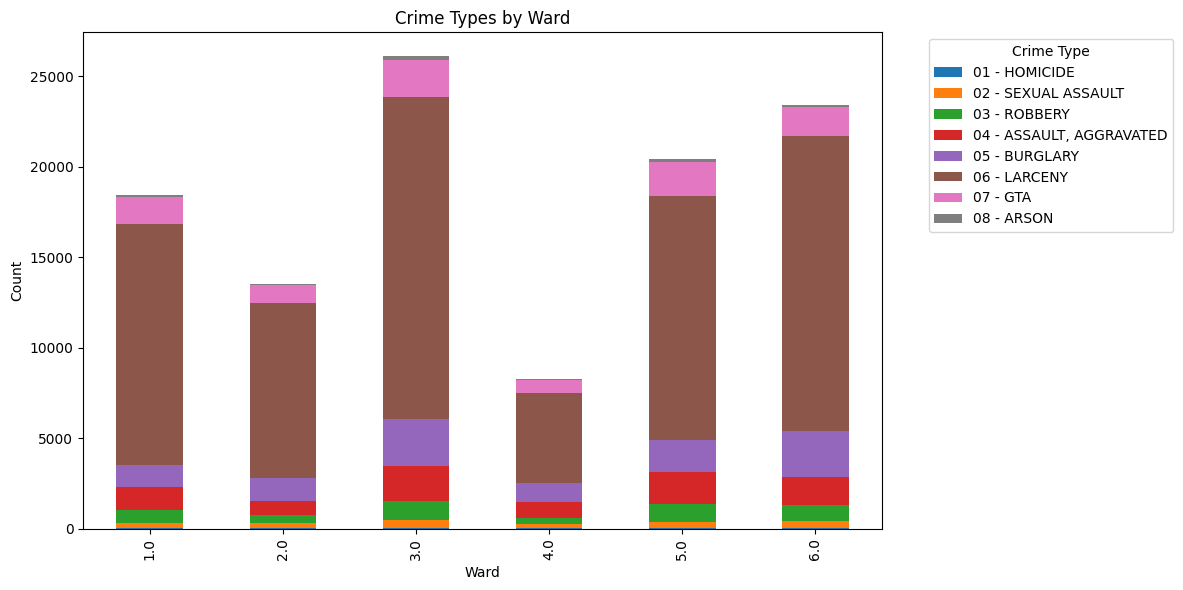
\includegraphics[keepaspectratio=true,scale=.6]{crime-types-by-ward}
    \caption{Prevelance of Crime Type per Ward}
    \label{fig:crime-type-by-ward}
  \end{center}
\end{figure}

\newpage
\section{Crime Types by Time}
\par The second stacked bar chart, “Crime Types by Time Period” (Figure \ref{fig:crime-type-by-time}), categorizes incidents into four daily time periods: Morning, Afternoon, Evening, and Night. Consistent with the ward-based analysis, Larceny again emerges as the most common crime in every time period. The Afternoon period shows the highest overall crime count, exceeding 35,000 incidents, while Nighttime reports the lowest, at approximately 15,000.

Although violent crimes such as Robbery and Assault account for a slightly larger share of incidents at Night compared to other times, their overall numbers remain relatively low. This suggests that while violent crimes are somewhat more likely to occur during nighttime hours, they do not significantly shift the overall crime landscape.

The high incidence of Larceny during the Afternoon and Evening may be linked to greater public activity during those hours, which increases opportunities for theft. In terms of mitigation, these findings suggest that increasing streetlight density could specifically help deter nighttime Robbery and Assault, though such efforts may have limited impact on overall crime, given Larceny's dominance and its timing.


\newpage
\begin{figure}[h]
  \begin{center}
    \advance\leftskip-3cm
    \advance\rightskip-3cm
    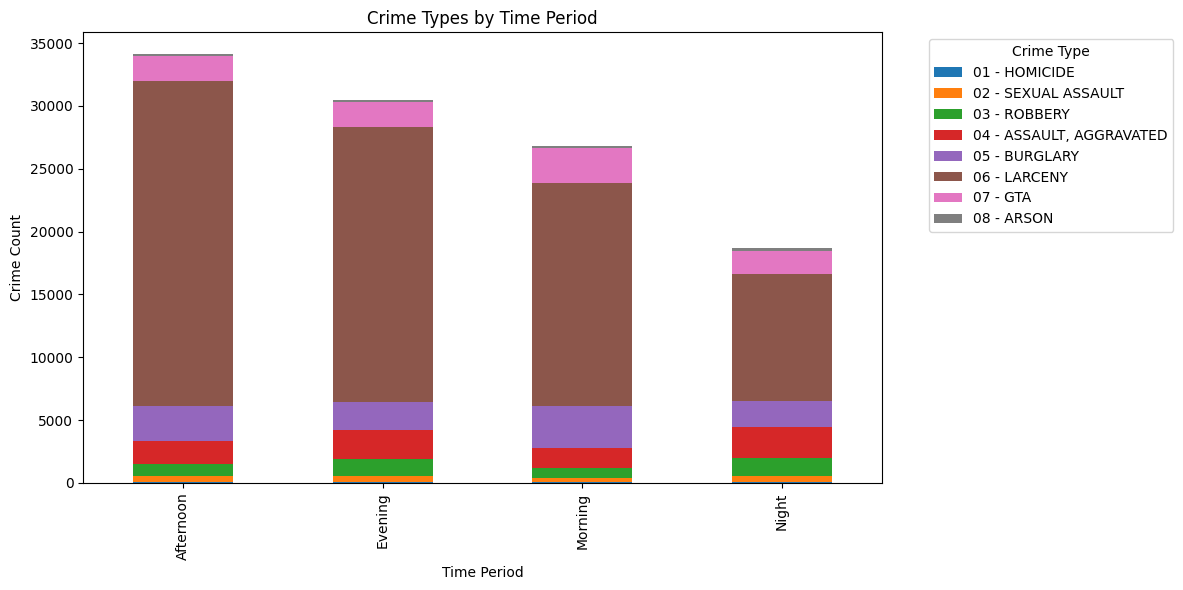
\includegraphics[keepaspectratio=true,scale=.6]{crime-types-by-time}
    \caption{Prevelance of Crime Type by Time Period}
    \label{fig:crime-type-by-time}
  \end{center}
\end{figure}


\par To further refine this temporal analysis, the histogram “Crime Count by Hour of Day” in Figure \ref{fig:crime-by-hour}, provides a granular view of crime distribution across the 24-hour cycle. Crime counts remain low from midnight to 6 AM, typically below 2,000 incidents, reflecting reduced activity during these hours. A sharp increase begins around 7 AM, peaking between 10 AM and 2 PM with counts exceeding 6,000 incidents, indicating a midday surge likely driven by Larceny and other opportunistic crimes. The count gradually declines after 2 PM but remains elevated through the evening, with a secondary peak around 6 PM to 8 PM, aligning with the Evening period’s high Larceny rates. Post-10 PM, crime counts taper off, consistent with the lower Night period totals. The kernel density curve smooths these trends, confirming a bimodal pattern with peaks at midday and early evening. This hourly breakdown reinforces the time period analysis, suggesting that crime prevention efforts should focus on peak activity hours, particularly 10 AM to 8 PM, while night-specific interventions like streetlighting could target the post-10 PM decline to further reduce residual crime

\begin{figure}[ht]
  \begin{center}
    \advance\leftskip-3cm
    \advance\rightskip-3cm
    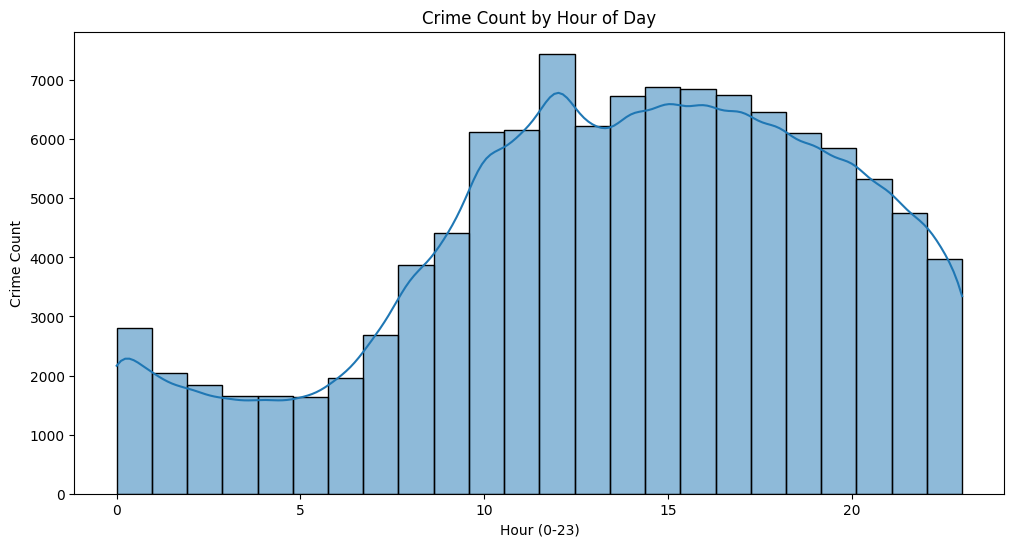
\includegraphics[keepaspectratio=true,scale=.6]{crime-by-hour}
    \caption{Total Crimes per Hour Throughout the 24 Hour Period}
    \label{fig:crime-by-hour}
  \end{center}
\end{figure}



\newpage
\section{Correlation Matrix Heatmap}
\par The heatmap provided in Figure \ref{fig:heatmap} is a correlation matrix that illustrates the relationships between various variables: median household income (MEDHINC\_CY), average household income (AVGHINC\_CY), streetlight count (Streetlight\_Count), crime count (Crime\_Count), arrest count (Arrest\_Count), and the proportion of nighttime crimes (Night\_Crime\_Prop). The color intensity and values (ranging from $-1.0$ to $1.0$) indicate the strength and direction of the correlation, with positive values showing a direct relationship and negative values indicating an inverse relationship.



\begin{figure}[ht!]
  \begin{center}
    \advance\leftskip-3cm
    \advance\rightskip-3cm
    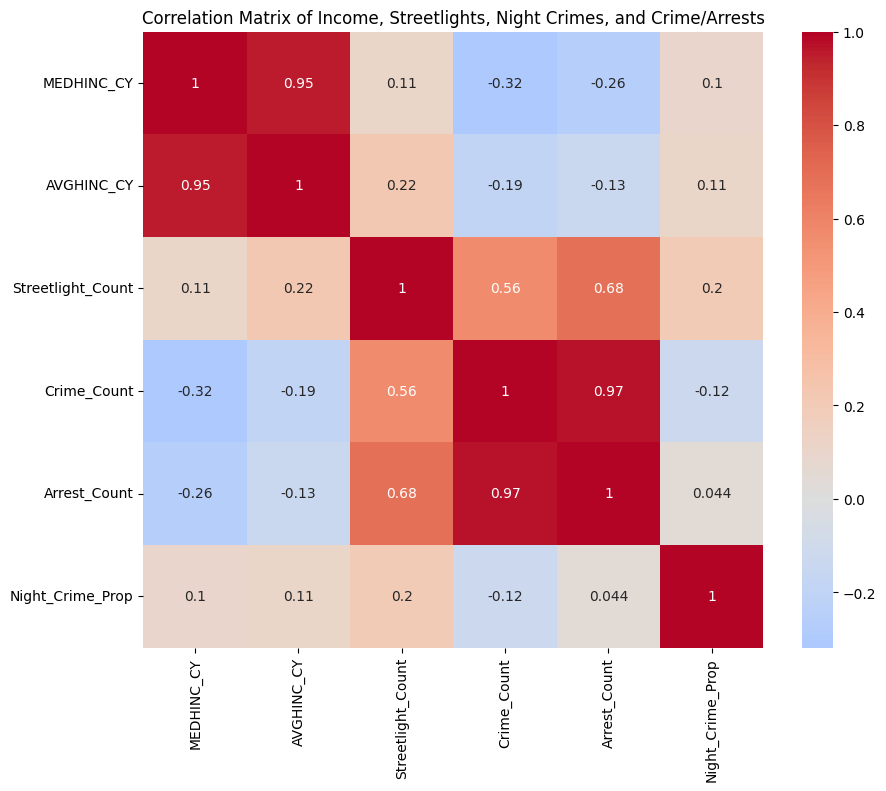
\includegraphics[keepaspectratio=true,scale=.6]{heatmap}
    \caption{Correlation Matrix Heatmap}
    \label{fig:heatmap}
  \end{center}
\end{figure}

\subsection{Key Insights}

\begin{itemize}
\item \textbf{Income vs. Crime and Arrests}
  \par MEDHINC\_CY and AVGHINC\_CY exhibit a strong positive correlation with each other ($0.95$), indicating that median and average incomes in neighborhoods are highly consistent. Both MEDHINC\_CY and AVGHINC\_CY have moderate negative correlations with Crime\_Count ($-0.32$ and $-0.19$, respectively) and Arrest\_Count ($-0.26$ and $-0.13$, respectively). This suggests that higher income levels are associated with lower crime and arrest rates, though the relationship is not extremely strong.
\item \textbf{Streetlights vs. Crime}
  \par Streetlight\_Count has a moderate positive correlation with Crime\_Count ($0.56$) and Arrest\_Count ($0.68$), indicating that areas with more streetlights tend to have higher crime and arrest numbers. There is a weak positive correlation between Streetlight\_Count and Night\_Crime\_Prop ($0.20$), suggesting a slight tendency for more streetlights to be associated with a higher proportion of nighttime crimes. The correlation between Streetlight\_Count and income variables ($0.11$ with MEDHINC\_CY, $0.22$ with AVGHINC\_CY) is weak, implying that streetlight presence is not strongly tied to income levels.
\item \textbf{Crime and Arrests}
  \par Crime\_Count and Arrest\_Count are strongly positively correlated ($0.97$), indicating that areas with more reported crimes also tend to have more arrests. Night\_Crime\_Prop has a weak positive correlation with Crime\_Count ($0.044$) and Arrest\_Count ($0.12$), suggesting that the proportion of nighttime crimes does not strongly drive overall crime or arrest rates.
\end{itemize}

\section{Exploratory Data Analysis Conclusion}
\par The exploratory analysis reveals significant insights into crime distribution across Tucson’s six wards and time periods. Larceny consistently dominates as the most prevalent crime type, particularly in high-crime wards like Ward 3 and during afternoon and evening hours, suggesting a link to increased public activity. Violent crimes, such as Aggravated Assault and Robbery, are more concentrated in wards 3 and 5, hinting at potential socioeconomic or environmental influences that warrant further investigation. The temporal analysis indicates a midday to early evening peak in crime, with a notable but smaller rise in violent crimes at night, supporting the potential role of streetlighting as a mitigation strategy. The correlation matrix highlights a moderate negative relationship between income and crime/arrest rates, while the positive correlation between streetlight count and crime suggests that lighting alone may not deter crime in areas with higher baseline activity. These findings lay a foundation for testing hypotheses about socioeconomic disparities and environmental impacts, guiding the subsequent modeling and policy recommendations.

\chapter{Results}


\begin{figure}[ht]
  \begin{center}
    \advance\leftskip-3cm
    \advance\rightskip-3cm
    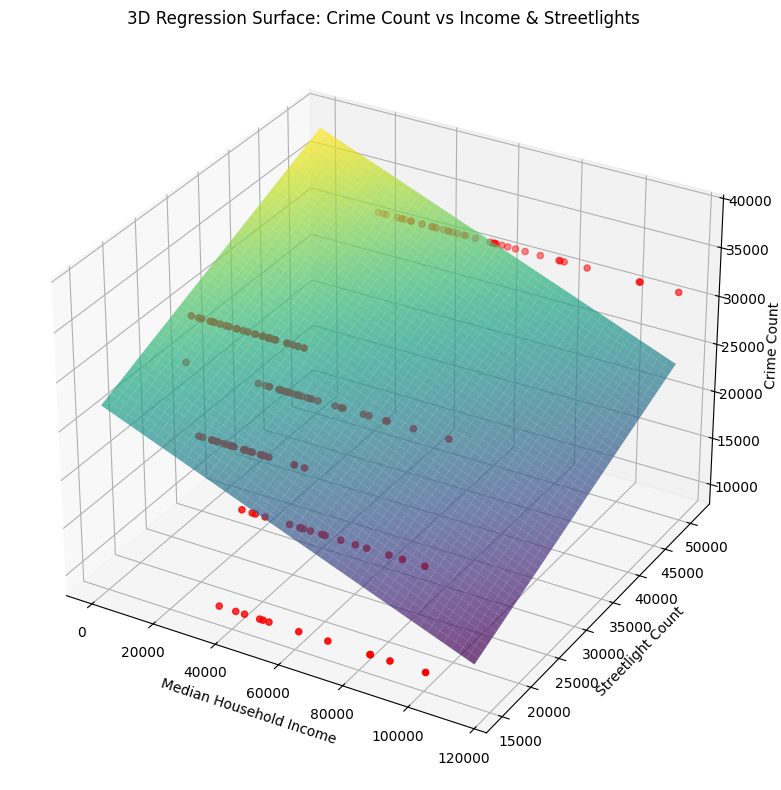
\includegraphics[keepaspectratio=true,scale=.5]{3d-cover}
    \caption{3D Regression Surface}
    \label{fig:3d-cover}
  \end{center}
\end{figure}


\newpage
\section{Ridge Regression}
\par We applied Ridge Regression, seen in Figure \ref{fig:ridge-reg}, to analyze hourly crime counts across four police divisions in Tucson—East, Midtown, South, and West—using the hour of the day as the independent variable. This technique introduces a regularization penalty to reduce model variance and avoid overfitting. The regression model was trained separately for each division, and we evaluated model performance using three metrics: $R^2$ score, Mean Absolute Error (MAE), and Mean Squared Error (MSE).

For each division, the model produced a linear equation of the form:

\begin{center}
  \begin{math}
    \text{CrimeCount} = \beta_0 + \beta_1(\text{Hour})
  \end{math}
\end{center}

where the coefficients $\beta_0$ and $\beta_1$ varied by division. For example, in the South Division—the area with the most pronounced upward trend—the slope coefficient was highest, indicating a sharp increase in crime as the day progresses. In contrast, Midtown and East had lower slope coefficients, suggesting a more moderate hourly increase.

The $R^2$ scores varied across divisions:
\begin{itemize}
\item \textbf{South Division} showed the strongest model fit with an $R^2$ value closest to 1, indicating that a large portion of the variance in crime count was explained by the hour of the day.
\item \textbf{East and Midtown Divisions} had moderate $R^2$ scores, suggesting the model captured the general upward trend but not all variability.
\item \textbf{West Division} exhibited the lowest $R^2$ score among the four, largely due to the higher variance in observed crime counts that the linear model could not fully account for.
\end{itemize}

MAE and MSE followed similar patterns. South Division had the lowest errors, reinforcing the strength of the model in that area. West Division had the highest error values, confirming the model's limited ability to account for the spread in crime counts, especially during peak hours.

Overall, Ridge Regression, seen in Figure \ref{fig:ridge-reg}, successfully modeled the general trend of increasing crime throughout the day. However, the variability in model performance across divisions suggests that linear models may not be sufficient for capturing more complex patterns, particularly in areas with higher variance. Future analyses could explore nonlinear models or include additional predictors (e.g., day of the week or crime type) to enhance predictive accuracy.

\newpage
\begin{figure}[h!]
  \begin{center}
    \advance\leftskip-3cm
    \advance\rightskip-3cm
    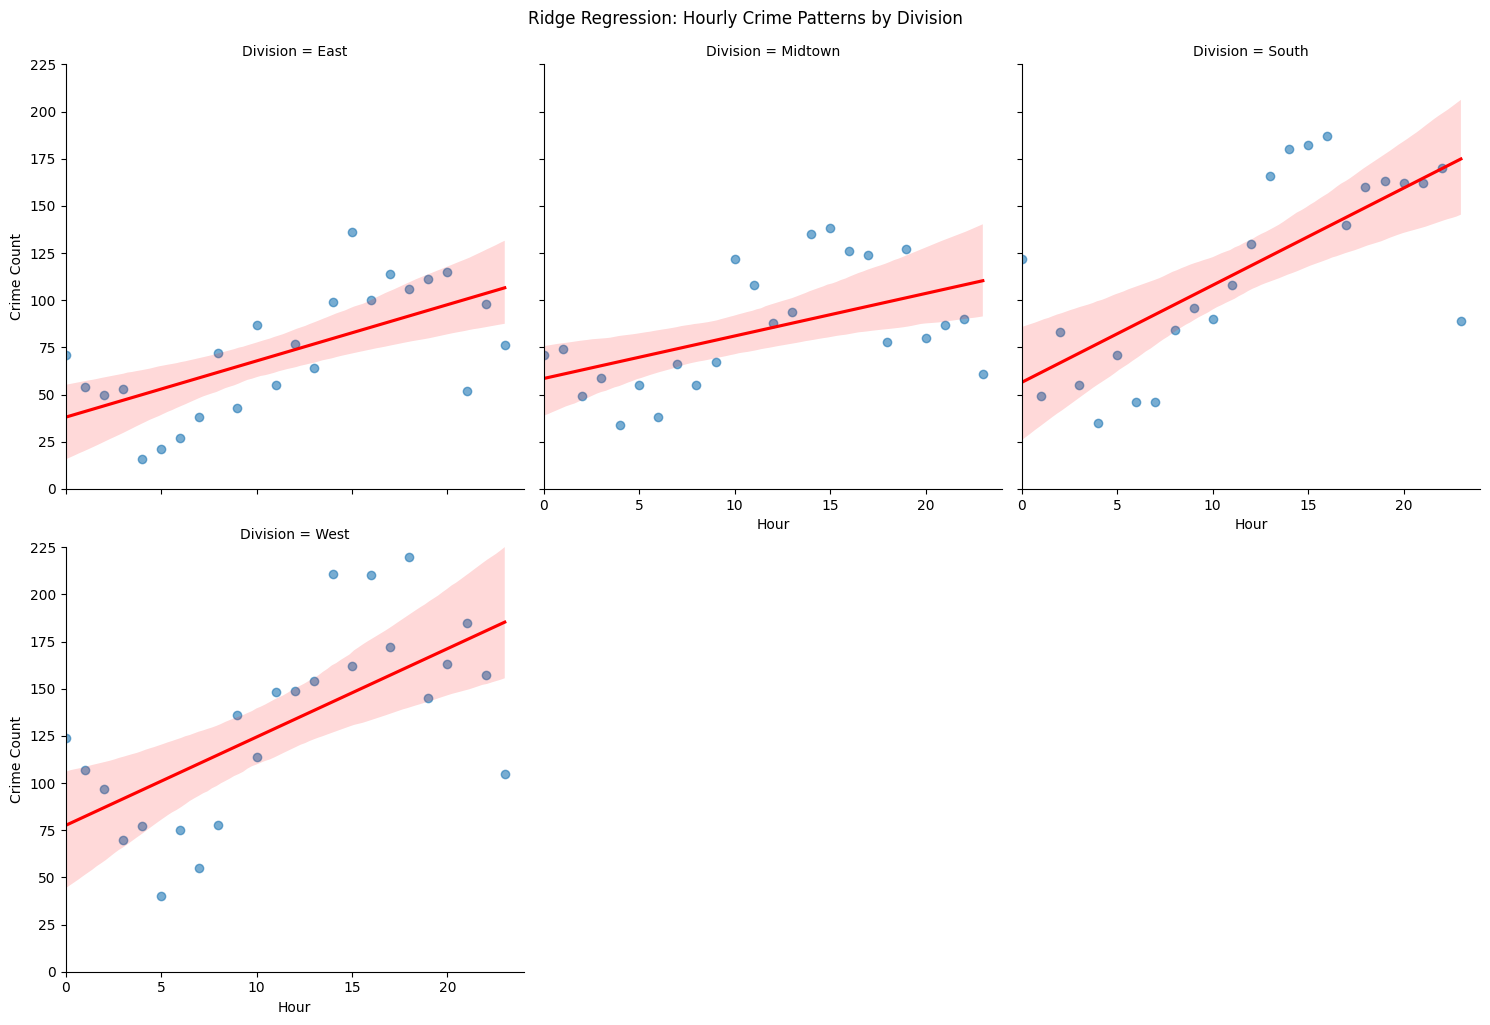
\includegraphics[keepaspectratio=true,scale=.5]{ridge-reg}
    \caption{Ridge Regression}
    \label{fig:ridge-reg}
  \end{center}
\end{figure}

\newpage
\section{Model Performance Evaluation}
\par The Random Forest (RF) and Logistic Regression (LR) models were evaluated to predict high-crime wards based on median household income (MEDHINC\_CY), average household income (AVGHINC\_CY), and streetlight presence (Streetlight\_Count). Performance metrics including accuracy, F1-score, and detailed classification reports are presented below.

\subsection{Random Forest Performance}
\par This section implements RF and LR models to predict whether a ward has a high crime rate, using predictors related like income, streetlight presence, and crime timing. It also evaluates model performance and interprets which features are most important.

\par The Random Forest model achieved an accuracy of 0.97 and an F1-score of 0.95, indicating strong predictive performance. The classification report is summarized in Table \ref{tab:rf_classification_report}.


\begin{table}[h!]
  \centering
  \caption{Random Forest Classification Report}
  \label{tab:rf_classification_report}
  \begin{tabular}{lcccc}
    \toprule
    & Precision & Recall & F1-Score & Support \\
    \midrule
    Class 0 (Low Crime) & 1.00 & 0.95 & 0.98 & 22 \\
    Class 1 (High Crime) & 0.91 & 1.00 & 0.95 & 10 \\
    \midrule
    Accuracy & \multicolumn{3}{c}{0.97} & 32 \\
    Macro Avg & 0.95 & 0.98 & 0.96 & 32 \\
    Weighted Avg & 0.97 & 0.97 & 0.97 & 32 \\
    \bottomrule
  \end{tabular}
\end{table}

\subsection{Logistic Regression Performance}
The Logistic Regression model yielded an accuracy of 0.75 and an F1-score of 0.71, performing less effectively than the Random Forest model. The classification report is detailed in Table~\ref{tab:lr_classification_report}.

\begin{table}[h!]
\centering
\caption{Logistic Regression Classification Report}
\label{tab:lr_classification_report}
\begin{tabular}{lcccc}
\toprule
 & Precision & Recall & F1-Score & Support \\
\midrule
Class 0 (Low Crime) & 1.00 & 0.64 & 0.78 & 22 \\
Class 1 (High Crime) & 0.56 & 1.00 & 0.71 & 10 \\
\midrule
Accuracy & \multicolumn{3}{c}{0.75} & 32 \\
Macro Avg & 0.78 & 0.82 & 0.75 & 32 \\
Weighted Avg & 0.86 & 0.75 & 0.76 & 32 \\
\bottomrule
\end{tabular}
\end{table}

\subsection{Feature Importance Analysis}
The Random Forest model's feature importance analysis revealed that the number of streetlights (Streetlight\_Count) was the most influential predictor of high-crime wards, with an importance score of approximately 0.5. Median household income (MEDHINC\_CY) and average household income (AVGHINC\_CY) followed, with importance scores around 0.25 each. This suggests that the presence of streetlights has a stronger association with crime rates compared to income levels, providing partial support for the hypothesis that streetlight presence influences crime rates. However, the income-related features still contribute meaningfully, indicating that wealth levels in neighborhoods also play a role in predicting crime, aligning with the hypothesis that thefts and violent crimes may vary between richer and poorer areas.
\par The Random Forest model outperformed Logistic Regression in predicting high-crime wards, with higher accuracy and F1-scores. The feature importance analysis highlights the significant role of streetlight presence in predicting crime rates, suggesting that urban infrastructure may influence crime more than socioeconomic factors like income in this dataset. These findings support the hypothesis that streetlight presence impacts crime rates and indicate a moderate relationship between crime and neighborhood wealth levels.

\section{Regression Analysis Results}

\par This section presents the results of two Ordinary Least Squares (OLS) regression models to analyze the impact of Median Household Income (MEDHINC\_CY) and Streetlight Count (Streetlight\_Count) on Crime Count. The models address the hypotheses: (1) whether thefts and violent crimes occur more often in richer or poorer neighborhoods, and (2) whether the presence of streetlights influences crime rates.

\subsection{Model 1: Crime Count vs Median Household Income}
\par The first OLS regression model, seen in Figure \ref{fig:cime-count-income}, examines the relationship between Crime Count and Median Household Income (MEDHINC\_CY). The model summary is presented in Table~\ref{tab:model1_summary}.

\newpage
\begin{table}[h!]
\centering
\caption{OLS Regression Summary}
\label{tab:model1_summary}
\begin{tabular}{lccccc}
\toprule
 & Coefficient & Std. Error & t-value & P-value & 95\% Conf. Interval \\
\midrule
Constant & 30690 & 1244.395 & 24.662 & 0.000 & [28240, 33140] \\
MEDHINC\_CY & -0.1067 & 0.025 & -4.199 & 0.000 & [-0.157, -0.057] \\
\midrule
\multicolumn{6}{l}{R-squared: 0.101, Adjusted R-squared: 0.095} \\
\multicolumn{6}{l}{F-statistic: 17.63, Prob (F-statistic): 4.48e-05} \\
\bottomrule
\end{tabular}
\end{table}

\par The negative coefficient for MEDHINC\_CY (-0.1067, p $<$ 0.001) indicates a statistically significant inverse relationship between median household income and crime count. As median income increases by one unit, crime count decreases by approximately 0.1067 units, supporting Hypothesis 1 that crime rates are higher in poorer neighborhoods. The R-squared value of 0.101 suggests that 10.1\% of the variance in crime count is explained by median household income alone, indicating a modest but significant relationship. The scatterplot of Crime Count vs Median Household Income visually confirms this downward trend, showing higher crime counts at lower income levels.


\begin{figure}[h!]
  \begin{center}
    \advance\leftskip-3cm
    \advance\rightskip-3cm
    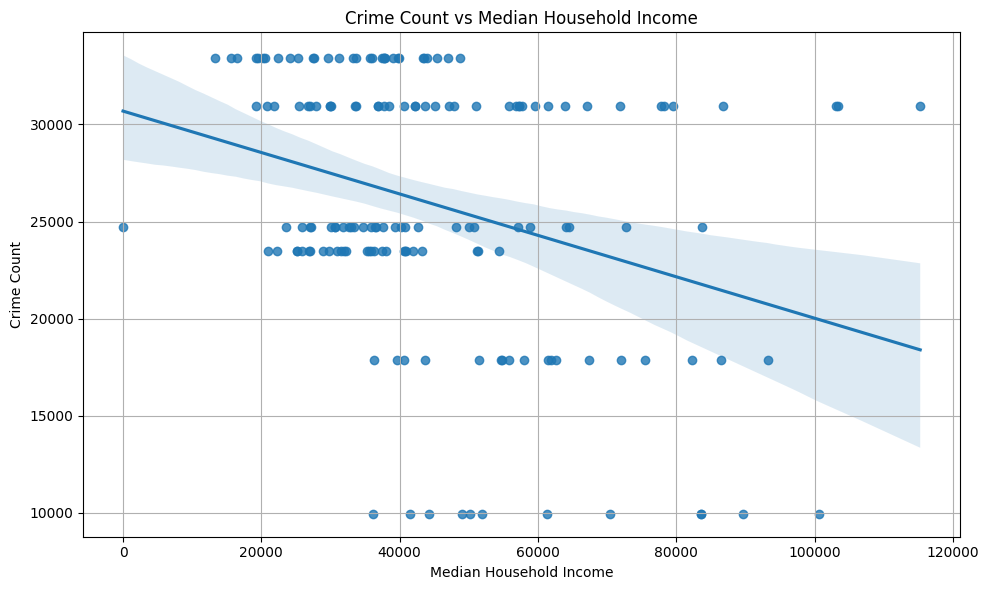
\includegraphics[keepaspectratio=true,scale=.6]{cime-count-income}
    \caption{Crime Count vs Median Household Income}
    \label{fig:cime-count-income}
  \end{center}
\end{figure}

\newpage
\subsection{Model 2: Crime Count vs Median Household Income and Streetlight Count}
The second OLS regression model, seen in Figure \ref{fig:3d-cover}, includes both Median Household Income (MEDHINC\_CY) and Streetlight Count as predictors of Crime Count. The model summary is shown in Table~\ref{tab:model2_summary}.


\begin{table}[h!]
\centering
\caption{OLS Regression Summary: Crime Count vs Median Household Income and Streetlight Count}
\label{tab:model2_summary}
\begin{tabular}{lccccc}
\toprule
 & Coefficient & Std. Error & t-value & P-value & 95\% Conf. Interval \\
\midrule
Constant & 22560 & 1252.670 & 18.010 & 0.000 & [20100, 25020] \\
Streetlight\_Count & 0.3069 & 0.030 & 10.205 & 0.000 & [0.247, 0.366] \\
MEDHINC\_CY & -0.1281 & 0.020 & -6.454 & 0.000 & [-0.167, -0.089] \\
\midrule
\multicolumn{6}{l}{R-squared: 0.461, Adjusted R-squared: 0.454} \\
\multicolumn{6}{l}{F-statistic: 66.67, Prob (F-statistic): 1.18e-21} \\
\bottomrule
\end{tabular}
\end{table}

\par This model shows improved explanatory power with an $R^2$ of 0.461, indicating that 46.1\% of the variance in crime count is explained by the combination of median household income and streetlight count. Both predictors are statistically significant (p $<$ 0.001). The coefficient for Streetlight\_Count (0.3069) suggests a positive relationship with crime count, meaning that an increase in streetlights is associated with an increase in crime, which is contrary to Hypothesis 2 that streetlight presence reduces crime rates. The coefficient for MEDHINC\_CY (-0.1281) remains negative and significant, reinforcing the finding from Model 1 that higher income is associated with lower crime counts. The 3D regression surface plot illustrates this relationship, showing a downward slope with respect to median household income and an upward slope with respect to streetlight count.

\subsection{Discussion}
\par The regression analysis provides insights into the relationships between crime count, median household income, and streetlight presence. Model 1 confirms Hypothesis 1, showing that crime counts are higher in poorer neighborhoods, as evidenced by the significant negative coefficient for MEDHINC\_CY. Model 2, however, challenges Hypothesis 2: while the Random Forest feature importance analysis (from the previous section) highlighted Streetlight\_Count as the most influential predictor, the positive coefficient in the OLS model suggests that areas with more streetlights experience higher crime counts. This could indicate that streetlights are more commonly installed in high-crime areas as a response to crime, rather than as a deterrent. The combined explanatory power of income and streetlight count in Model 2 ($R^2$ = 0.461) underscores the importance of considering both socioeconomic and infrastructural factors when analyzing crime patterns.

\begin{thebibliography}{9}
\bibitem{welsh08}
  Welsh, B.C. and Farrington, D.P. (2008), Effects of Improved Street Lighting on Crime. Campbell Systematic Reviews, 4: 1-51. https://doi.org/10.4073/csr.2008.13
\bibitem{jr07}
  HIPP, J.R. (2007), INCOME INEQUALITY, RACE, AND PLACE: DOES THE DISTRIBUTION OF RACE AND CLASS WITHIN NEIGHBORHOODS AFFECT CRIME RATES?*. Criminology, 45: 665-697. https://doi.org/10.1111/j.1745-9125.2007.00088.x
\end{thebibliography}

\end{document}
